\section{Software Design}
\phantomsection
\subsection{UML Modeling}

In this chapter are specified and documented the artifacts of MyApp system using UML diagrams. UML can be described as a general purpose visual modeling language to visualize, construct, specify and document software system. The diagrams are aim to help developers, business users and anybody interested to understand the system. To model a system the most important aspect is to capture the dynamic behaviour. There are five diagrams in UML available to model it: use case, sequence, state and activity diagram. However, class and deployment diagram are also important to examine. They represent physical and conceptual elements of the system that are present in MyApp platform as nodes and classes.

Use case diagrams are used to gather the requirements of the MyApp system including internal and external agets known as actors. There is only one actor -- user -- that interacts with the system. The system functionalities are captured in use cases as shown in the Figure \ref{usecase_uml}.

\begin{figure}[!ht]
\centering
\includegraphics[width=15cm]{usecase}
\caption{Use Case Diagram}\label{usecase_uml}
\end{figure}

There are not so many use cases, because the core processes that made the application running where executed in backend. Thus, the user are using only the system functionalities. First use case represents the primary functionality of the system handled by search engine. 

The use case diagrams specify the events of the system and their flows, but never describes how they are implemented. To fulfill this sequence diagrams are used. Moreover, they captures the time sequence of messages flow from one object to another. 

Since it uses objects to show the messages flow and objects are derived from classes, the sequence diagrams are dependent upon class diagrams. Thus, first will be shown the class diagrams and after that the sequence ones. 

The class diagrams help us to model and analyse the static views of the application. Through them the responsabilities of the system are described. Each class entity has its own methods and attributes. In the Figure \ref{classCreate_uml} are shown the classes responsabile for database creation. 

\begin{figure}[!ht]
\centering
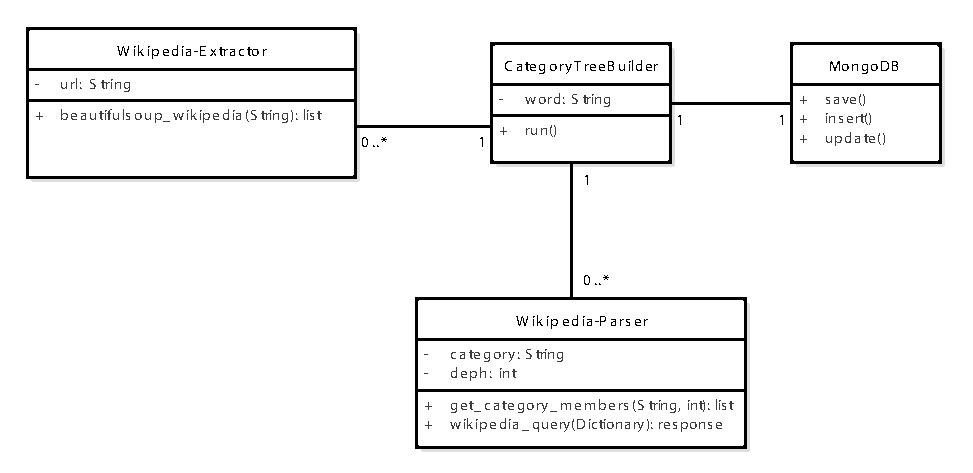
\includegraphics[width=16cm]{create-db}
\caption{Database Creation Class Diagram}\label{classCreate_uml}
\end{figure}

The \textit{CategoryTreeBuilder} class is responsible for setting the order of methods to be called in order to create the database. First the \textit{Wiki\_Extractor} calss is called, which has the responsiblity to extract the web page from the given url. The class \textit{Wikipedia\_Parser} has two attributes and two methods that are working with wikipedia API. Thus, the class is responsible to request particular "actions" by specifying an action parameter, mainly "action=query" to get information.. \textit{MongoDB} class has the task to save the records to database according to the model.  

Structure of database model is shown in Figure \ref{classMongo_uml}

\begin{figure}[!ht]
\centering
\includegraphics[width=16cm]{mongo-db}
\caption{MongoDB Models Class Diagram}\label{classMongo_uml}
\end{figure}

Although it has a simple structure, the mongodb document is well structured. \textit{Category} holds the industry for which the category tree is composed. \textit{Subcategories} holds an array of embedded documents that contain the fields \textit{name} and \textit{subcategory\_tree}. The subcategory\_tree field is an array of strings. 

A more complex class diagram is build for MapReduce framework used for word frequency count. It has five classes responsible for creating a parallel, distributed algorithm on a cluster for processing large data sets. For MyApp the local machine will act as Server and as Client at the same time. The relations between classes are shown in Figure \ref{hadoop_uml}.

\begin{figure}[!ht]
\centering
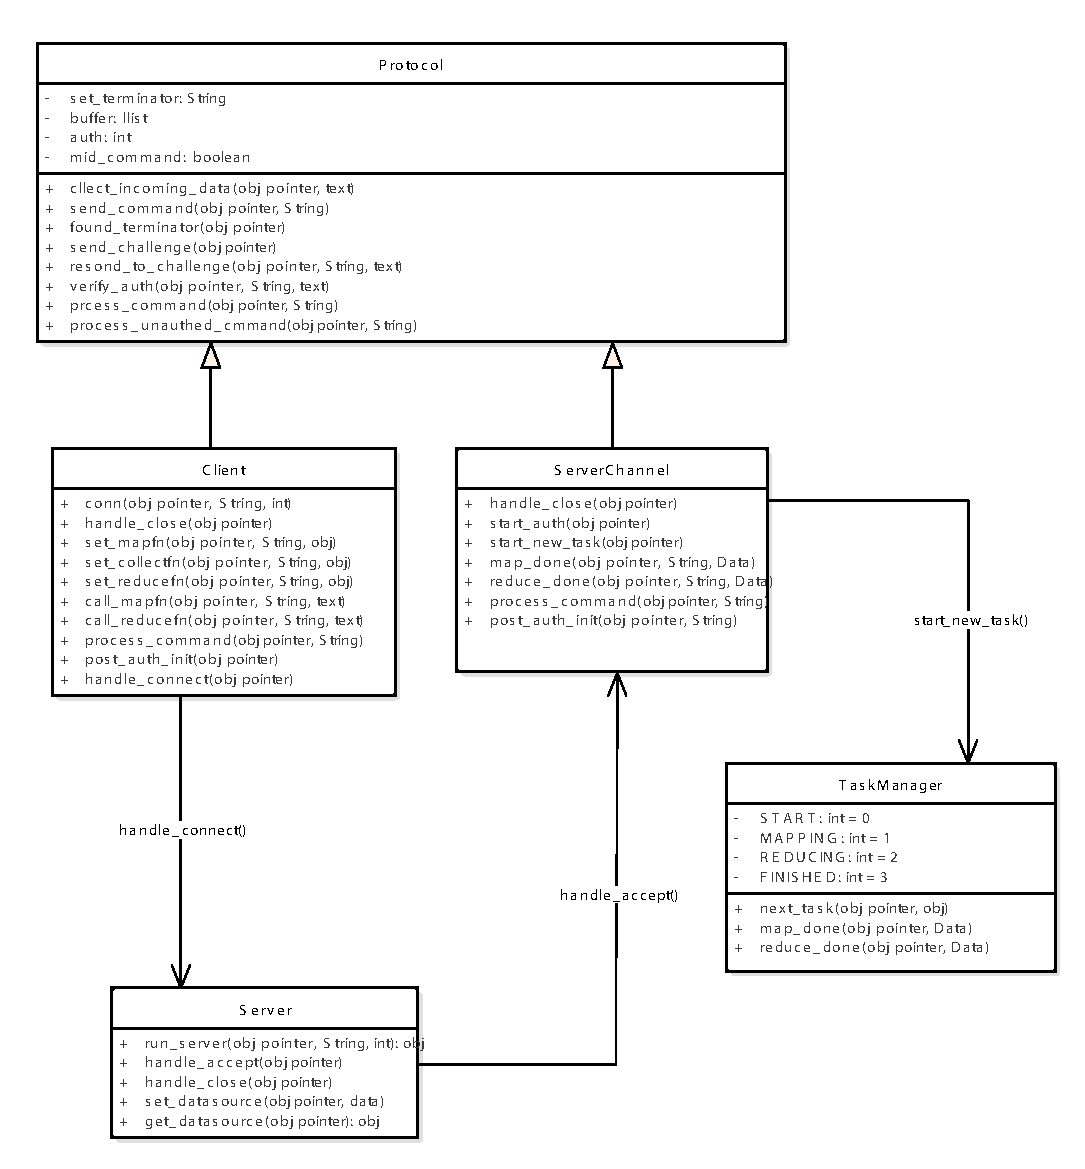
\includegraphics[width=16cm]{hadoop}
\caption{MapReduce Class Diagram}\label{hadoop_uml}
\end{figure}


Now, when all the main classes for MyApp system are documented the sequence diagrams can be created. The sequence diagrams listed below are only for main processes of the running system at a particular moment. 

In the Figure \ref{createDB_uml} is described the process of creation the categories database. The sequence diagram is having four objects Execute, Wikipedia-Extractor, Wikipedia-Parser and MongoDB, detailed described in Figure \ref{classCreate_uml}.

\begin{figure}[!ht]
\centering
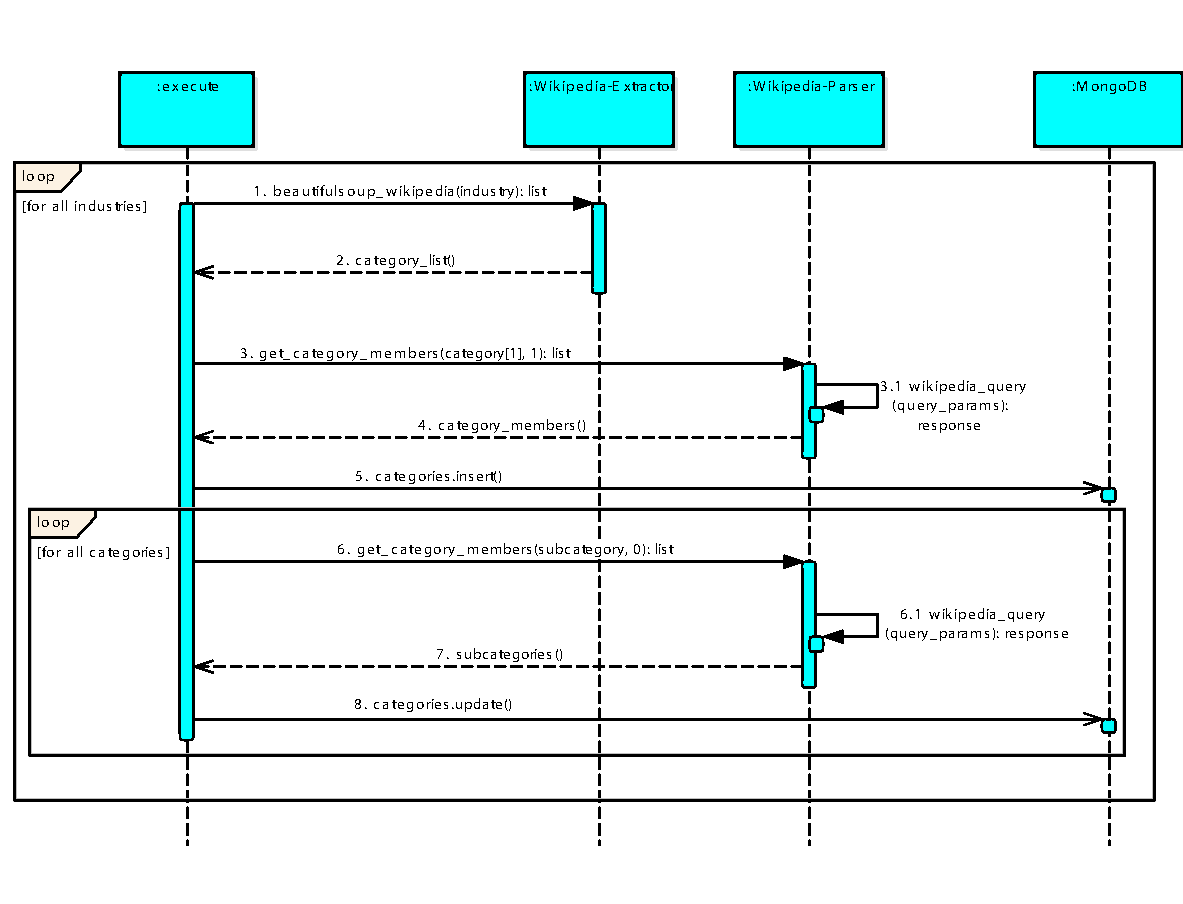
\includegraphics[width=16cm]{CreateDB}
\caption{Database Creation Sequence Diagram}\label{createDB_uml}
\end{figure}

The first call is \textit{beautifulsoup\_wikipedia(industry)} wich is a method of \textit{Wikipedia-Extractor} object. The method returns a list of categories for the given industry. The next call is \textit{get\_category\_members(catgeory[1], 1)} which is also a method of \textit{Wikipedia-Extractor} object. To return a response the \textit{Wikipedia-Extractor} object executes a self call \textit{wikipedia\_query}. After this a list of all category members is returned. The returned list is stored in different documents of Mongo database through the call \textit{categories.insert()}.

Since the last return was a list of categories members, the next calls are executed in a loop. The loop control structure is represented in the diagram as a fragmanet with the condition: for all categories. 

First call in the loop is the same method of the object \textit{Wikipedia-Extractor} explained above -- \textit{get\_category\_members(subcategory, 0)} but with different parameters. The last call here is \textit{categories.update()} which is method of \textit{MongoDB} object. It updates the documents of the database with additional inofrmation from the return list. 

The whole proceess of database creation is executed in a loop for all industries that requires category tree. 

Another important diagram that describes the dynamic aspects of the MyApp system is activity diagram. It shows the flow from one activity to another activity. For a better understanding of the described flow swimlanes are used. They group activities performed by the same thread as showm in Figure \ref{doc_uml}. 

\begin{figure}[!ht]
\centering
\includegraphics[width=15cm]{document-classification}
\caption{MapReduce Activity Diagram}\label{doc_uml}
\end{figure}
















 






